\section{Introduction}

This chapter contains an evaluation of the performance of OmniTune
when tasked with selecting workgroup size of SkelCL stencil codes. The
effectiveness of each of the autotuning techniques described in the
previous chapter are scrutinised and evaluated using multiple
different machine learning algorithms, and the prediction quality is
evaluated for portability across programs, devices, and datasets.


\subsubsection{Questions to ask of each approach to autotuning}

\begin{enumerate}
\item How successful is it at selecting optimal workgroup sizes?
\item How successful is it at selecting \emph{good} workgroup sizes?
\item What is the performance when training on synthetic benchmarks
  and testing on real?
\item What is the performance when testing on an unseen: architecture,
  kernel, dataset? (leave one out evaluation)
\item How well does it perform as a function of the number of training
  points?
\end{enumerate}


\section{Runtime Results}

This section presents the results of the empirical enumeration of
workgroup size optimisation space for SkelCL stencils. A total of
\input{gen/num_runtime_stats} combinations of scenario and workgroup
size were tested, distributed across \input{gen/num_scenarios}
scenarios, with an average of \input{gen/num_avg_params} unique
workgroup sizes each. % FIXME: (max \input{gen/num_max_params}).

\subsection{Statistical soundness}

\begin{figure}
\begin{subfigure}[h]{.32\textwidth}
\centering
\includegraphics{gen/img/runtimes_histogram_1}
\vspace{-1.5em} % Shrink vertical padding
\caption{}
\label{fig:runtimes-histogram-1}
\end{subfigure}
~%
\begin{subfigure}[h]{.32\textwidth}
\centering
\includegraphics{gen/img/runtimes_histogram_2}
\vspace{-1.5em} % Shrink vertical padding
\caption{}
\label{fig:runtimes-histogram-2}
\end{subfigure}
~%
\begin{subfigure}[h]{.32\textwidth}
\centering
\includegraphics{gen/img/runtimes_histogram_3}
\vspace{-1.5em} % Shrink vertical padding
\caption{}
\label{fig:runtimes-histogram-3}
\end{subfigure}
\\
\begin{subfigure}[h]{.32\textwidth}
\centering
\includegraphics{gen/img/runtimes_histogram_4}
\vspace{-1.5em} % Shrink vertical padding
\caption{}
\label{fig:runtimes-histogram-4}
\end{subfigure}
~%
\begin{subfigure}[h]{.32\textwidth}
\centering
\includegraphics{gen/img/runtimes_histogram_5}
\vspace{-1.5em} % Shrink vertical padding
\caption{}
\label{fig:runtimes-histogram-5}
\end{subfigure}
~%
\begin{subfigure}[h]{.32\textwidth}
\centering
\includegraphics{gen/img/runtimes_histogram_6}
\vspace{-1.5em} % Shrink vertical padding
\caption{}
\label{fig:runtimes-histogram-6}
\end{subfigure}
\\
\begin{subfigure}[h]{.32\textwidth}
\centering
\includegraphics{gen/img/runtimes_histogram_7}
\vspace{-1.5em} % Shrink vertical padding
\caption{}
\label{fig:runtimes-histogram-7}
\end{subfigure}
~%
\begin{subfigure}[h]{.32\textwidth}
\centering
\includegraphics{gen/img/runtimes_histogram_8}
\vspace{-1.5em} % Shrink vertical padding
\caption{}
\label{fig:runtimes-histogram-8}
\end{subfigure}
~%
\begin{subfigure}[h]{.32\textwidth}
\centering
\includegraphics{gen/img/runtimes_histogram_9}
\vspace{-1.5em} % Shrink vertical padding
\caption{}
\label{fig:runtimes-histogram-9}
\end{subfigure}

\caption{%
  Distribution of runtimes for 6 test cases, with increasing mean
  runtimes between 2-200ms (shown with a horizontal dashed line). Each
  plot shows a histogram of 1000 observations with a fitted kernel
  density estimate.%
}
\label{fig:runtime-histograms}
\end{figure}

\begin{figure}
\centering
\includegraphics{gen/img/ci_trend}
\caption{%
  % TODO: Use \input{gen/max_ci} and \input{gen/mean_ci}
  Ratio of confidence interval to mean as a function of sample
  count. The two dashed lines indicate the confidence interval at the
  minimum sample count (4.6\%), and mean sample count (2.8\%).%
}
\label{fig:ci-trends}
\end{figure}


\begin{figure}
  \centering
\begin{subfigure}[h]{.45\textwidth}
  \centering
  \includegraphics{gen/img/num_samples}
  \caption{}
\end{subfigure}
\hfill
\begin{subfigure}[h]{.45\textwidth}
  \centering
  \includegraphics{gen/img/num_params}
  \caption{}
\end{subfigure}

\caption{Breakdown of number of}
\label{fig:num-samples}
\end{figure}


A total of \input{gen/num_samples} runtimes were recorded, with an
average of \input{gen/avg_sample_count} runtimes per test case (min
\input{gen/min_sample_count}). Figure~\ref{fig:sample-counts} shows
the sample count per test cases. Figure~\ref{fig:min-max-runtimes}
shows the distribution of minimum and maximum runtimes for each
combination of scenario and workgroup size.

\TODO{Actually demonstrate that differences in runtime between
  measured workgroup sizes are significant.}


\subsection{Assessing Available Performance}

By comparing the relative performance of different workgroup sizes
across workloads, we can begin to get a feel for the real performance
impact. From the set of all workgroup sizes $W$, the subset of
workgroup sizes $W_{legal}(s) \subseteq W$ that are legal for a given
scenario $s$ can be found using:

\begin{equation}
  W_{legal}(s) = \left\{w | w \in W, w < W_{max}(s) \right\} - W_{refused}(s)
\end{equation}

Where $W_{max}(s)$ is the maximum workgroup size constraints imposed
by the scenario device and kernel. Given a function $t(s,w)$ which
returns the arithmetic mean of the measured runtimes for a given
scenario $s$ and workgroup size $w$, we can calculate the speedup
$r(s, w_1, w_2)$ of competing workgroup sizes $w_1$ over $w_2$ using:

\begin{equation}
  r(s, w_1, w_2) = \frac{t(s,w_2)}{t(s,w_1)}\\
\end{equation}


\subsubsection{Oracle Workgroup Size}

For a given scenario, the \emph{oracle} workgroup size
$\Omega(s) \in W_{legal}(s)$ is the $w$ value which provided the
lowest mean runtime. This allows for comparing the performance of a
particular workgroup against the maximum available performance for
that scenario:

\begin{align}
  \Omega(s) &= \argmin_{w \in W_{legal}(s)} t(s,w)\\
  p(s,w) &= r(s, w, \Omega(s))
\end{align}

Where the performance is within the range $0 \le p(s,w) \le 1$. The
geometric mean is used to aggregate relative performances due to it's
multiplicative property~\cite{Fleming1986}. For a given workgroup
size, the average performance $\bar{p}(w)$ across the set of all
scenarios $S$ can be found using the geometric mean of performance
relative to the oracle:

\begin{equation}
\bar{p}(w) =
\left(
  \prod_{s \in S} r(s, w, \Omega(s))
\right)^{1/|S|}
\end{equation}


\subsubsection{Performance Upper Bounds}

\begin{figure}
\begin{subfigure}[h]{\textwidth}
\centering
\includegraphics{gen/img/max_speedups.pdf}
\caption{%
  Worst workgroup size.%
}
\label{fig:oracle-speedups-worst}
\end{subfigure}
\\
\begin{subfigure}[h]{\textwidth}
\centering
\includegraphics{gen/img/oracle_speedups.pdf}
\caption{%
  Best static workgroup size.%
}
\label{fig:oracle-speedups-baseline}
\end{subfigure}

\caption{%
  Two comparisons of the performance of the oracle workgroup size for
  each scenario relative to: (\subref{fig:oracle-speedups-worst})~the
  worst workgroup size for each scenario; and
  (\subref{fig:oracle-speedups-baseline})~the workgroup size which
  provides the best average case performance across all scenarios.%
}
\label{fig:speedups}
\end{figure}

For a given scenario $s$, the ratio of the workgroups sizes from
$W_{legal}(s)$ which provide the longest and shortest mean runtimes
can be used to calculate the upper bound of the possible performance
influence of workgroup size:

\begin{equation}
r_{max}(s) = r(s, \argmax_{w \in W_{legal}(s)} t(s,w), \Omega(s))
\end{equation}

When applied to each scenario $s \in S$ from the experimental results,
the range of performance upper bounds is found to be
$\input{gen/min_possible_speedup}\times$ -
$\input{gen/max_possible_speedup}\times$ (geometric mean
$\input{gen/avg_possible_speedup}\times$). Figure~\ref{fig:oracle-speedups-worst}
shows the maximum attainable speedups achieved for all scenarios.


\subsubsection{Establishing a Baseline}

The \emph{baseline} workgroup size $\bar{w}$ is the value which
provides the best average case performance across all scenarios.  By
defining $W_{safe} \in W$ as the intersection of legal workgroup
sizes, the baseline can be found using:

\begin{align}
W_{safe} &= \cap \left\{ W_{legal}(s) | s \in S \right\}\\
\bar{w} &= \argmax_{w \in W_{safe}} \bar{p}(w)
\end{align}

From the experimental results, the baseline workgroup size $\bar{w}$
is found to be \input{gen/one_r}, with a geometric mean performance
$\bar{p}(\bar{w})$ of
\input{gen/one_r_perf}. Figure~\ref{fig:oracle-speedups-baseline}
shows the average speedup of the oracle over this baseline for all
scenarios. If we assume that a pragmatic developer with enough time
would eventually find this static optimal, then this provides a
reasonable upper bound on the attainable improvements of an autotuner
for workgroup size over that of a static choice.


\subsubsection{Human Expert}

The stencil workgroup size as chosen by a human expert is
$32 \times 4$.


\subsection{Distribution of Oracle Workgroup Sizes}

\begin{figure}
\begin{subfigure}[t]{0.98\textwidth}
\centering
\includegraphics{gen/img/max_wgsizes.pdf}
\vspace{-1.5em} % Shrink vertical padding
\caption{}
\label{fig:max-wgsizes}
\end{subfigure}
\\
\begin{subfigure}[t]{0.98\textwidth}
\centering
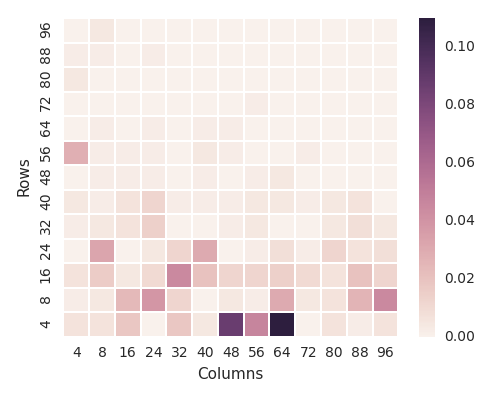
\includegraphics{gen/img/oracle_param_space.pdf}
\vspace{-1.5em} % Shrink vertical padding
\caption{}
\label{fig:oracle-wgsizes}
\end{subfigure}

\caption{%
  The distribution of: (\subref{fig:max-wgsizes}) maximum legal
  workgroup sizes, and (\subref{fig:oracle-wgsizes}) for all
  scenarios. The distribution of oracle workgroup sizes is uneven and
  spread across the space.%
}
\label{fig:heatmaps}
\end{figure}

Figure~\ref{fig:max-wgsizes} shows the distribution of maximum
workgroup sizes across all scenarios. Figure~\ref{fig:oracle-wgsizes}
shows the distribution of oracle workgroup sizes, demonstrating that
there is clearly no ``silver bullet'' workgroup size which works for
all scenarios. As Figure~\ref{fig:oracle-accuracy} shows,
\input{gen/num_wgsizes_50_accuracy} unique workgroup sizes are
required in order to achieve oracle performance just 50\% of the
time. \FIXME{These values are going to change massively once I'd
  incorporated the CPU data\ldots}

\begin{figure}
\centering
\includegraphics{gen/img/num_params_oracle.pdf}
\caption{%
  Accuracy compared to the oracle as a function of the number of
  workgroup sizes used. The best accuracy that is achievable using a
  single statically chosen value is
  \protect\input{gen/max_oracle_param_frequency}.%
}
\label{fig:oracle-accuracy}
\end{figure}

The mode of the oracle workgroup sizes is
\input{gen/max_oracle_param}, which is optimal for
\input{gen/max_oracle_param_frequency} of scenarios. Note that this is
a different value from the \emph{baseline} identified previously,
which identifies the single choice which provides the best average
case performance. This is because the value is not legal for all
scenarios; that is, $\input{gen/max_oracle_param_w} \not\in W_{safe}$.
Figure~\ref{fig:performance-legality} illustrates this point by
plotting the geometric mean performance across workgroup sizes for:
all scenarios, and only the scenarios for which the workgroup size is
legal.

\TODO{Partial baseline. How much performance could we get if we lock
  one of the parameters and twiddle the other?}

\begin{figure}
\centering
\includegraphics{gen/img/params_summary.pdf}
\caption{%
  The red line shows the ``legality'' of workgroup sizes, i.e.\ the
  ratio of scenarios for which that workgroup size is legal.  The blue
  and green lines show the geometric mean of the performance relative
  to the oracle for: all scenarios, and only the scenarios for which
  the workgroup size is legal.%
}
\label{fig:performance-legality}
\end{figure}


\begin{table}
  \parbox{.45\linewidth}{
    \centering
    \scriptsize
    \rowcolors{2}{white}{gray!25}
    \input{gen/tab/top_params_coverage}
    \caption{Ranked by legality.}
  }
  \hfill
  \parbox{.45\linewidth}{
    \centering
    \scriptsize
    \rowcolors{2}{white}{gray!25}
    \input{gen/tab/top_params_perf}
    \caption{Ranked by performance.}
  }
\end{table}


\subsection{Factors Influencing Workgroup Size Performance}

A common approach taken by application developers is to set the
workgroup size for a kernel based on the maximum legal workgroup size,
for example to use the square root of the maximum to set the number of
columns and rows. While the reasoning for this approach is perfectly
intuitive, these results indicate that there no useful correlation
between the ratio of a particular workgroup size to the maximum legal
workgroup and the observed performance, as shown in
Figure~\ref{fig:performance-wgsizes}. Furthermore, the performance of
workgroup sizes is shown in Figure~\ref{fig:performances} to be vary
greatly across architectures, kernels, and datasets.

\TODO{Go into some detail here about the knock-on effect that changing
  workgroup size has on memory utilisation and execution unit
  occupancy.}

\begin{figure}
\begin{subfigure}[h]{\textwidth}
\centering
\includegraphics{gen/img/performance_max_wgsize}
\vspace{-1.5em} % Shrink vertical padding
\caption{}
\label{fig:performance-max-wgsize}
\end{subfigure}
\\
\begin{subfigure}[h]{.48\textwidth}
\centering
\includegraphics{gen/img/performance_max_c}
\vspace{-1.5em} % Shrink vertical padding
\caption{}
\label{fig:performance-wg-c}
\end{subfigure}
~%
\begin{subfigure}[h]{.48\textwidth}
\centering
\includegraphics{gen/img/performance_max_r}
\vspace{-1.5em} % Shrink vertical padding
\caption{}
\label{fig:performance-wg-r}
\end{subfigure}

\caption{%
  Comparing workgroup performance relative to the oracle as function
  of: (\subref{fig:performance-max-wgsize})~maximum legal size,
  (\subref{fig:performance-wg-c})~number of columns, and
  (\subref{fig:performance-wg-r})~ number of rows. As can be seen,
  workgroup size alone is not indicative of performance. \FIXME{Shit
    plots.}%
}
\label{fig:performance-wgsizes}
\end{figure}

\begin{figure}
\begin{subfigure}[h]{\textwidth}
\centering
\includegraphics{gen/img/performance_kernels.pdf}
\vspace{-1.5em} % Shrink vertical padding
\caption{Kernels}
\label{fig:performance-kernels}
\end{subfigure}
\\
\begin{subfigure}[h]{.48\textwidth}
\centering
\includegraphics{gen/img/performance_devices.pdf}
\vspace{-1.5em} % Shrink vertical padding
\caption{Devices}
\label{fig:performance-devices}
\end{subfigure}
~%
\begin{subfigure}[h]{.48\textwidth}
\centering
\includegraphics{gen/img/performance_datasets.pdf}
\vspace{-1.5em} % Shrink vertical padding
\caption{Datasets}
\label{fig:performance-datasets}
\end{subfigure}

\caption{%
  Performance relative to the oracle of workgroup sizes across all
  test cases, grouped by: (\subref{fig:performance-kernels})~kernels,
  (\subref{fig:performance-devices})~devices, and
  (\subref{fig:performance-datasets})~datasets.%
}
\label{fig:performances}
\end{figure}

By comparing the relative performance of an average of
\input{gen/num_avg_params} workgroup sizes for each workload, the
following conclusions can be drawn:

\begin{enumerate}
\item The performance of a workgroup size for a particular workload
  depends properties of the hardware, software, and dataset. The
  performance gap between different workgroup sizes for a single
  workload is up to $\input{gen/max_possible_speedup}\times$.
\item Not all workgroup sizes are legal, and we can only test if a
  value \emph{is} legal at runtime.
\item Differing workloads have wildly different optimal workgroup
  sizes, and the best performance can be achieved using static tuning
  is optimal for only \input{gen/max_oracle_param_frequency} of
  workloads.
\end{enumerate}

I believe this presents a compelling case for the development of an
autotuner which can select the optimal workgroup size at runtime.


\section{Classification Performance}

\begin{enumerate}
\item How often does it select \emph{invalid} workgroup sizes?
\item How does the three different techniques of handling invalid
  workgroup sizes perform?
\end{enumerate}

\begin{figure}
\centering
\includegraphics{gen/img/classification-xval.pdf}
\caption{%
  Classification performance using cross-validation.%
}
\end{figure}

\begin{figure}
\centering
\includegraphics{gen/img/classification-xval-random.pdf}
\caption{%
  Per-instance performances of classification using cross-validation
  and the ``random'' error handler.%
}
\end{figure}


% \TODO{Rank eigenvectors of PCA on features.}

% \TODO{Evaluate the effectiveness of training with synthetic
%   benchmarks.}


\section{Predicting Stencil Runtime}

\begin{enumerate}
\item How accurately does it predict the runtime of a stencil?
\item What is the relationship between \emph{classification} accuracy,
  and the accuracy of predicted runtimes? Does it really matter if the
  predicted runtime is inaccurate?
\end{enumerate}

\begin{figure}
\centering
\includegraphics{gen/img/runtime-regression-xval.pdf}
\caption{%
  Performance of regressors at predicting program runtime.%
}
\end{figure}


\section{Predicting Relative Performance}


\section{Summary}

\begin{table}
\scriptsize
\input{\DataDir/tab/xval.tex}
\caption{Results of 10 fold cross-validation.}
\end{table}

\begin{table}
\scriptsize
\input{\DataDir/tab/synthetic_real.tex}
\caption{Results of training using synthetic benchmarks and testing on
  real.}
\end{table}
